\section{Summary}
\label{sec:summary-4-relationship}

    From the open problem of \cite{Johansen16STstruct}, we have that there is no embedding between higher-dimensional automata and ST-structures. By introducing Chu spaces, we were able to define a translation between Chu spaces over $\mathbf{3}$ and ST-structures, and the translation can be used interchangeably. Also, Chu spaces over $\mathbf{3}$ are shown to be isomorphic to ST-structures.
    
    At the end of Section \ref{sec:Chu-spaces}, Chu spaces provided the notion of a sculpting method for higher-dimensional automata. A conjecture posed by Vaughan Pratt was that any higher-dimensional automata could be obtained using the sculpting method. As shown, we have that Chu spaces over $\mathbf{3}$ are isomorphic to ST-structures as well as there is no existing embedding between higher-dimensional automata and ST-structures. Hence, as the main result of our study, we show that not all higher-dimensional automata can be sculpted. We provide a diagram of the correlation between Chu spaces, ST-structures, Sculptures and higher-dimensional automata. In the diagram, we provide the propositions that prove the isomorphism between ST-structures and Chu spaces as well as ST-structures and Sculptures. Also, we provide the counter-example, see Example \ref{exp:hda-broken-box}, which shows a higher-dimensional automaton which is not a sculpture.
    
    
    From the result of Chu spaces over $\mathbf{3}$ being isomorphic to ST-structures, we will challenge Pratt's conjecture by developing an algorithm to decide whether an higher-dimensional automaton can be sculpted or not, and show several simple examples of \emph{acyclic} higher-dimensional automata which are not sculptures. We believe that this contradicts Pratt's conjecture. Below is a diagram of the propositions which show the correlation between Chu spaces, ST-structures and Sculptures. Together with a counter-example of the conjecture, showing a higher-dimensional automaton which is not a sculpture.
    
    
    %However, we still do not have a model that is capable to capture every aspect of higher-dimensional automata. Luckily, Pratt provided an intuition for a certain method of modelling processes from higher-dimensional automata. This method is called sculpting, and the model obtained is called a sculpture. Furthermore, Pratt made a conjecture that the method of sculpting could capture every aspect of higher-dimensional automata. We will define sculptures in the next chapter and challenge Pratt's conjecture by answering in negatives by giving examples of higher-dimensional automata which are not sculptures.

    \begin{center}
        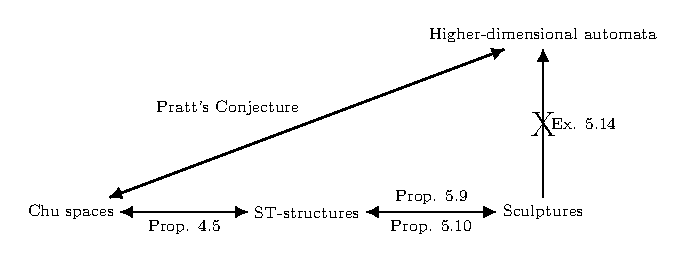
\includegraphics[scale=1]{Figures/4.Relationship-with-other-models-of-concurrency/Chu-spaces-and-ST-structures/argument-diagram.pdf}
    \end{center}
    
    We have shown a proof for Proposition \ref{prop:ST-structure-Chu-over-3}, but need to provide proofs for Proposition \ref{prop:ST-to-Sculpture} and Proposition \ref{prop:Sculpture-to-ST} to show the correlation between Chu spaces, Sculptures and ST-structures. In the next chapter, we will provide the remaining proofs needed to show both the counter-example of the conjecture and correlation of the models.